
\documentclass{article}
\usepackage{graphicx}
\graphicspath{ {HistoriaIMG} }

\usepackage[utf8]{inputenc}
\usepackage[T1]{fontenc}

\usepackage{microtype}
\usepackage{xurl}
\usepackage{hyperref}
\usepackage{csquotes}
\usepackage{multicol}
\usepackage{float}
\usepackage[numbers]{natbib}

\title{História da Fotografia}
\author{Laura Aidar}

\begin{document}
\maketitle

\begin{abstract}
Frases escolhidas com base na frequência de trigramas:
\begin{itemize}
\item Foi em meados do século X que o árabe Alhaken de Basora percebeu a natureza das imagens que se projetavam no interior de sua tenda trespassada pela luz solar.
\item Em 1871, o método de emulsão seca de brometo de prata em colódio foi aperfeiçoado pelo médico inglês Richard Leach Maddox (1816-1902), que substituiu o colódio por placas secas de gelatina.
\item Considerado o maior colecionador de fotografias do século XIX, Dom Pedro II não teve tempo de levar sua preciosa coleção para o exílio.
 
\end{itemize}
\end{abstract}

\section*{Entidades Nomeadas}
\begin{multicols}{4}
\begin{itemize}
\item A História da Fotografia (MISC)
\item Grécia Antiga (ORG)
\item Aristóteles (PER)
\item Alhaken de Basora (LOC)
\item Ângelo Sala (PER)
\item Sol (LOC)
\item Carl Wilhelm Scheele (PER)
\item Johann Henrich Schulze (PER)
\item Thomas Wedgwood (PER)
\item Joseph Niépce (PER)
\item Louis Jaques Mandé Daguerre (PER)
\item Academia de Ciências de Paris (ORG)
\item John F. Goddard (PER)
\item William Henry Fox Talbot (PER)
\item James Clerk Maxwell (PER)
\item Gabriel Lippman (PER)
\item Auguste (PER)
\item Louis Lumière (PER)
\item Ducos du Hauron (PER)
\item Richard Leach Maddox (PER)
\item Kodak (ORG)
\item Brownie-Kodak (ORG)
\item Kodak (ORG)
\item Kodachrome (MISC)
\item Polaroid (MISC)
\item Kodak (ORG)
\item DCS (ORG)
\item Louis Daguerre (PER)
\item Campinas (LOC)
\item SP (LOC)
\item Antoine Hercule Florence (PER)
\item Langsdorff (PER)
\item Brasil (LOC)
\item Boris Kossoy (PER)
\item Florence (PER)
\item Brasil (LOC)
\item França (LOC)
\item Louis Compte (PER)
\item Dom Pedro II (PER)
\item Brasil (LOC)
\item Marc Ferrez (PER)
\item Brasil (LOC)
\item Guerra do Paraguai (MISC)
\item Guerra de Canudos (MISC)
\item Flávio de Barros (PER)
\item Dom Pedro II (PER)
\item Biblioteca Nacional (LOC)
\item Imperatriz (LOC)
\item Teresa Cristina (PER)
\item Louis Daguerre (PER)
\item Academia de Ciências da França (ORG)
\item Estado (LOC)
\item História do Cinema

Cores Primárias (MISC)

\end{itemize}
\end{multicols}
\section{História da Fotografia}

A História da Fotografia estuda as imagens produzidas a partir da exposição de material fotossensível. Também estão incluídas as que foram captadas pelas lentes das modernas máquinas fotográficas digitais.

Igualmente, se ocupa em entender os diferentes aparelhos que possibilitaram reter a imagem e imprimi-la numa placa de vidro, metal, gelatina ou papel.

A origem etimológica de “fotografia” vem do grego e significa "gravar com luz": "foto" (luz) e "graphein" (escrever, gravar).



\section{Origem da Fotografia}

As primeiras experiências fotográficas de químicos e alquimistas datam da antiguidade.

Na Grécia Antiga, foi criado um aparelho chamado "câmera obscura", capaz de criar imagens invertidas. Ele é considerado o precursor das câmeras fotográficas. A autoria do dispositivo é comumente atribuída a Aristóteles. O aparelho foi sendo ajustado e usado por artistas e cientistas até a invenção da fotografia.


        \begin{figure}[H]
        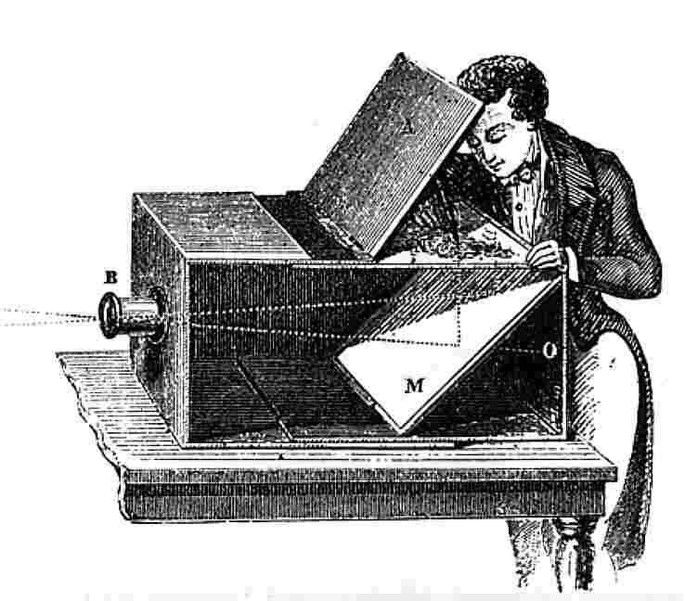
\includegraphics[width=\linewidth]{cameraescurahistoriadafotografia-cke.jpg}


        \caption{Ilustração do século XIX mostra pessoa usando uma câmera escura. Foto: domínio público}


        \end{figure}
        Foi em meados do século X que o árabe Alhaken de Basora percebeu a natureza das imagens que se projetavam no interior de sua tenda trespassada pela luz solar.

Em 1525, já se dominava a técnica de escurecimento dos sais de prata. No ano de 1604, o químico italiano Ângelo Sala (1576-1637) já sabia que alguns compostos de prata oxidavam quando expostos à luz do Sol.

Por sua vez, o farmacêutico sueco Carl Wilhelm Scheele (1742-1786) viria a contribuir com esta descoberta em 1777, ao demonstrar o enegrecimento de sais expostos à ação da luz.

No ano de 1725, foi a vez do cientista alemão Johann Henrich Schulze (1687-1744) projetar uma imagem durável numa superfície. Por conseguinte, o químico britânico Thomas Wedgwood (1771-1805) realizou no início do século XIX experimentos semelhantes.



\section{Evolução da Fotografia}

Muitos foram os pioneiros que pesquisaram como fixar uma imagem no papel. "Tirar fotografia", "fazer um retrato" tornou-se moda na segunda metade do século XIX.

A primeira fotografia propriamente dita foi obra do francês Joseph Niépce (1763-1828). Ele estudava as propriedades do cloreto de prata sobre papel desde 1817 e obteve sua grande obra no verão de 1826.


        \begin{figure}[H]
        
\includegraphics[width=\linewidth]{primeirafotografiadomundo-cke.jpg}


        \caption{Essa é a considerada a primeira fotografia do mundo, produzida por Niépce}


        \end{figure}
        \subsection*{Daguerreótipo}

Por sua vez, outro francês, Louis Jaques Mandé Daguerre (1789-1851), desenvolveu alguns anos depois o aparelho que leva seu nome, o “daguerreótipo”, capaz de gravar imagens permanentes.

O equipamento foi apresentado à Academia de Ciências de Paris em 1839, ano que entrou para a história como um marco para a fotografia.


        \begin{figure}[H]
        
\includegraphics[width=\linewidth]{daguerreotipo-cke.jpg}


        \caption{O daguerreótipo era uma caixa enorme que captava a imagem através da lente e a gravava sobre o vidro}


        \end{figure}
        Entretanto, o daguerreótipo tinha alguns problemas, como seu peso, o que dificultou sua popularização.

\subsection*{Calótipo}

Em 1840, o químico inglês John F. Goddard (1795-1866), criou lentes com maior abertura. No ano seguinte, o escritor e cientista inglês William Henry Fox Talbot (1800-1877) criou o "calótipo", aperfeiçoando o processo de fixação de imagens.


        \begin{figure}[H]
        
\includegraphics[width=\linewidth]{calotipo-cke.jpg}


        \caption{Exemplo de imagem obtida através do calótipo: o negativo, à esquerda e o positivo, à direita}


        \end{figure}
        \subsection*{Fotografia colorida}

A primeira fotografia colorida seria criada alguns anos depois, em 1861, pelo físico escocês James Clerk Maxwell (1831-1879).

Contribuíram nesta empreitada Gabriel Lippman (1845-1921), os irmãos Auguste (1862-1954) e Louis Lumière (1864-1948). Mais tarde, os irmãos conseguiriam colocar as imagens em movimento, fato que daria origem ao cinema.

Por fim, o francês Ducos du Hauron (1837-1920) desenvolveu uma forma de imprimir três negativos com filtros coloridos em vermelho e azul.


        \begin{figure}[H]
        
\includegraphics[width=\linewidth]{fotografiacoloridabb-cke.jpg}


        \caption{Primeira fotografia feita por Ducos du Hauron, em Agen, em 1877. Ao fundo, a catedral de Saint-Caprais}


        \end{figure}
        Em 1871, o método de emulsão seca de brometo de prata em colódio foi aperfeiçoado pelo médico inglês Richard Leach Maddox (1816-1902), que substituiu o colódio por placas secas de gelatina.



\section{Popularização da fotografia}

Durante o século XIX, a fotografia começa a fazer parte do dia a dia, mas apenas os fotógrafos profissionais, que trabalhavam em estúdios, conseguiam comprar um aparelho.

A fotografia passou a registrar momentos específicos como casamentos, aniversários e solenidades públicas. Para que tudo ficasse perfeito, os fotografados deveriam permanecer imóveis a fim de que a imagem fosse captada e impressa no papel.


        \begin{figure}[H]
        
\includegraphics[width=\linewidth]{brownie2overview-cke.jpg}


        \caption{Este é o segundo modelo portátil da Brownie-Kodak que permitiu a difusão da fotografia}


        \end{figure}
        Um marco histórico foi o ano de 1901, quando a empresa americana Kodak lançou a Brownie-Kodak, uma câmera comercial e popular.

Em 1935, a Kodak introduziria o Kodachrome, o pioneiro na linha de filmes coloridos. Nesta linha, a também americana Polaroid cria a fotografia colorida instantânea em 1963.

\subsection*{Digitalização da fotografia}

Outra inovação da Kodak seria a criação da câmera digital DCS 100 em 1990, uma máquina digital de fácil manipulação e barata.

Aqui se inicia uma era de gravações digitais de imagens a partir de uma câmera digital ou de telefones celulares. Sem o suporte do papel, as imagens podem ser armazenadas em computadores ou na web, para serem editadas, impressas e difundidas.



\section{História da fotografia no Brasil}


        \begin{figure}[H]
        
\includegraphics[width=\linewidth]{pacoimperial1840-cke.jpg}


        \caption{A imagem do atual Paço Imperial feita por Louis Compte em 1840 é uma das primeiras realizadas no Brasil}


        \end{figure}
        \subsection*{Surgimento da fotografia no Brasil}

Ao mesmo tempo que Louis Daguerre realiza seus experimentos, outro francês, radicado em Campinas (SP), busca fixar as imagens numa superfície. Trata-se de Antoine Hercule Florence (1804-1879), um viajante que participou da expedição científica de Langsdorff e que decidiu fazer do Brasil seu novo lar.

Graças às pesquisas do historiador Boris Kossoy, sabemos que Florence utilizou, inclusive, a palavra "fotografia" em 1832, bem antes que muitos dos seus colegas europeus.

Desta maneira, vemos que a fotografia não foi uma invenção isolada, mas fruto de vários pesquisadores, que perseguiam o mesmo objetivo ao mesmo tempo.

\subsection*{Incentivo de Dom Pedro II à fotografia}

Oficialmente, porém, a fotografia chega ao Brasil em 1840, apenas um ano após a invenção do daguerreótipo na França.

O abade francês Louis Compte fez demonstrações ao então jovem imperador Dom Pedro II, que fica maravilhado com o invento. O soberano passou a colecionar daguerreótipos, posava constantemente para retratos e inclusive teve diversos fotógrafos oficiais que deixaram inúmeros registros da família imperial e do Brasil.

A partir da urbanização e do crescimento das grandes cidades, a fotografia ganha seu espaço na sociedade brasileira. Podemos citar o fotógrafo Marc Ferrez (1843-1923) que realizou inúmeros registros e ainda hoje é uma referência de profissional do século XIX.

No entanto, a fotografia no Brasil serviu para deixar registrados momentos dramáticos como a Guerra do Paraguai (1865-1870) e a Guerra de Canudos (1895). Ambos os conflitos passaram pelas lentes de Flávio de Barros.



\section{Curiosidades sobre a fotografia}

\begin{itemize}
\item{Considerado o maior colecionador de fotografias do século XIX, Dom Pedro II não teve tempo de levar sua preciosa coleção para o exílio. Meses mais tarde, doou seu acervo de mais de 25 mil imagens à Biblioteca Nacional, com uma condição: que o conjunto levasse o nome da Imperatriz Teresa Cristina.}
\item{O dia da Fotografia é celebrado em 19 de agosto quando o francês Louis Daguerre apresenta seu invento na Academia de Ciências da França, em 1839. No mesmo ano, o Estado francês declara o daguerreótipo como um bem de domínio público.}
\end{itemize}

Gostou? Temos mais textos para você:

\begin{itemize}
\item{História do Cinema}
\item{Cores Primárias}
\item{Fotorrealismo}
\end{itemize}




\section*{Artigo Original}
Laura Aidar, História da Fotografia: \url{https://www.todamateria.com.br/historia-da-fotografia/}
\end{document}
